\documentclass[10pt]{article}
\usepackage[T1]{fontenc}
\usepackage[utf8]{inputenc}
\usepackage[margin=0.85in]{geometry}
\usepackage{amsmath}
\usepackage{amssymb}
\usepackage{booktabs}
\usepackage{array}
\usepackage{graphicx}
\usepackage{float}
\usepackage{placeins}
\usepackage{tabularx}
\usepackage{longtable}
\usepackage{hyperref}
\hypersetup{colorlinks=true,linkcolor=blue!50!black,citecolor=blue!50!black,urlcolor=blue!50!black}
\usepackage{xcolor}
\graphicspath{{figures/}}

\title{Machine-Learning Models for Skipper-CCD Noise Prediction:\\ Technical Reference}
\author{ML-assisted optimization of CCD operating parameters --- reference document}
\date{22 October 2026 (code state of commit \texttt{c7d7a65} and later)}
\newcommand{\code}[1]{\texttt{#1}}
\newcommand{\se}{\sigma_e}
\emergencystretch=3em
\sloppy
\hbadness=10000
\newcolumntype{L}{>{\raggedright\arraybackslash}X}

\begin{document}
\maketitle

\begin{abstract}
This is the reference for every machine-learning model in the repository and for everything around them: how a packet
becomes training data, how the inputs are prepared, the exact form of every model (kernels, priors, networks, training
settings, how the mean and the error bar are produced), how features are chosen, how the models are validated and
compared, how feature importance is learned, and the synthetic world on which every result so far was obtained. Every
statement is taken from the code (\code{lvl1/train\_lvl1.py}, \code{src/ml/*.py}, \code{src/process\_packet.py},
\code{lvl1/feature\_study.py}, \code{lvl1/feature\_importance.py}) and the file and function are named, so that each
model can be re-implemented or audited. The design discussion and the history of the results are in
\code{docs/overleaf\_ml\_models/ml\_models.tex}; the beginner's explanations in \code{docs/overleaf\_ml\_guide/}.
\end{abstract}

\tableofcontents

%======================================================================
\section{Conventions}
\label{sec:conv}

\begin{itemize}
  \item \textbf{One example} = one amplifier (board, channel) in one packet. A packet read by 4 amplifiers gives 4
        examples. The examples of a packet share the CCD's state and are never split between training and test.
  \item \textbf{Targets} $Y = (\log\se, \log\lambda, \log g)$, natural logs: $\se$ in e$^-$, $\lambda$ in e$^-$ per
        pixel (bin) per image, $g$ in ADU/e$^-$. An error of $0.05$ in a log is a 5\,\% relative error.
  \item \textbf{Label errors} $Y_{\rm err}$ are relative errors (WADERs' error divided by the value), used as standard
        deviations in log units (first order).
  \item \textbf{Settings} $\theta$: the operating parameters the boards report for the packet (\code{theta.*} columns).
  \item \textbf{Own features}: the trace features of the amplifier at $\theta$ (\code{X\_trace}) and at the reference
        settings taken in the same packet (\code{X\_ref}). The amplifier's identity (board, channel) is \emph{never} a model
        input, except in the labelled reference model \code{physics\_hier} (Section~\ref{sec:physics}).
  \item \textbf{Every model} has the interface \code{fit(X, Y)} and \code{predict(X)} $\to$ (mean, std), both of shape
        $(n, 3)$ in log units; std is the model's own 1-$\sigma$ predictive uncertainty.
  \item \textbf{Fold-local fitting}: every standardization, imputation and every learned quantity uses the training rows
        of the fold only. The only exceptions are label-free and are stated where they occur (the packet state from a test
        packet's own rows, the pre-training on unlabeled curves, the label-free cover order of the feature ladder).
\end{itemize}

%======================================================================
\section{From a packet to the model inputs}
\label{sec:data}

\subsection{Processing one packet (\code{src/process\_packet.py})}

\begin{enumerate}
  \item \textbf{Traces.} Every trace is decoded (\code{decode\_trace}), checked (\code{quality\_problems()}: a trace with
        lost data is marked unusable and gets no features), split into regions (\code{trace\_regions.split\_regions}) and
        reduced to 141 scalars and 18 curves (\code{trace\_features.trace\_features}; implementation tiers 0/1/2 =
        85/29/27 scalars). Per trace and feature the value is the median over the usable pixels.
  \item \textbf{Repeated trace sets} of one (kind $\in$ \{theta, ref\}, board, channel) are combined
        (\code{combine\_repeats}): the \emph{mean} over the usable repeats, after dropping, when at least 5 repeats are
        finite (\code{MIN\_REPEATS\_FOR\_REJECTION}), every value with $|v - \mathrm{median}| > 5 \times 1.4826\,
        \mathrm{MAD}$ (\code{REJECT\_ROBUST\_SIGMA}); the standard deviation over the kept repeats ($\mathrm{ddof}=1$) is
        stored as \code{trace\_sd.*}. Curves are combined as the per-point median over the usable sets
        (\code{ml/real\_inputs.per\_row\_curves}).
  \item \textbf{Labels} (\code{extract\_labels}): WADERs fits the pixel-charge distribution with
        $\mathrm{Norm}\sum_k \mathcal N(x; \mu_0 + k g, \sigma)\,\mathrm{Poisson}(k;\lambda)$ and writes
        \code{MEGAIN}$=g$, \code{MESIG}$=\sigma$ (ADU), \code{MEDC}$=\lambda g$ (ADU). Then
        \[ \se = \frac{\mathrm{MESIG}}{\mathrm{MEGAIN}},\qquad \lambda = \frac{\mathrm{MEDC}}{\mathrm{MEGAIN}},\qquad
           \delta\se = \sqrt{(\delta\sigma/g)^2 + (\sigma\,\delta g/g^2)^2}, \]
        and likewise for $\lambda$. A label is \emph{flagged} (\code{label.ok} = false) when a parameter is within 0.1\,\%
        of the range from its fit limit, when an error is zero or below $10^{-4}$ of the value (not for the gain), when an
        error exceeds half the value (not for $\mu$), or when a key is missing.
  \item \textbf{Per-row dark charge} (\code{src/image\_rows.py}): per image row, $\lambda_r$ by maximum likelihood with
        WADERs' $g$ and $\sigma$ fixed ($k = 0\dots6$, pedestal = median of the pixels within $3\sigma$ of the 0-e$^-$
        peak, error from the curvature); then a weighted straight line
        \[ \lambda_r = \mathrm{CIC} + \mathrm{DC}\,x_r,\qquad x_r = \frac{r + 1/2}{R/2}, \]
        through the $R$ rows in readout order, giving \code{label.lambda\_dark} (DC), \code{label.lambda\_cic} and their
        $2\times2$ covariance (strongly anti-correlated).
  \item \textbf{Dataset} (\code{dataset\_rows}): one row per (packet, board, channel) with \code{theta.*},
        \code{delta.*} (change from the reference), \code{label.*}, \code{trace.*}, \code{ref.*}, \code{trace\_sd.*},
        \code{ref\_sd.*}, \code{diff.*} = trace $-$ ref, \code{image.*} (FITS header, e.g.\ \code{image.NDCM}).
\end{enumerate}

\subsection{The model-input files (\code{src/ml/real\_inputs.py}, \code{build\_all})}

Nothing is fitted in this step (no standardization, no imputation), so nothing leaks between folds. One file per model
family in \code{<processed>/model\_inputs/}; shapes for $n$ examples, $p$ settings, $f$ features, $C$ curves.

\begin{table}[H]
\centering\small
\begin{tabularx}{\textwidth}{>{\raggedright\arraybackslash}p{2.4cm}>{\raggedright\arraybackslash}p{4.6cm}L}
\toprule
file & arrays (shape) & notes \\
\midrule
common part (every labelled file) & \code{packet\_id} $(n)$, \code{board} $(n)$, \code{channel} $(n)$, \code{amplifier} $(n)$,
\code{Y} $(n,3)$, \code{Y\_err} $(n,3)$, \code{targets} (3), \code{label\_ok} $(n)$, \code{fake} $(n)$, \code{theta} $(n,p)$,
\code{theta\_names} $(p)$ & $Y = \log$ of the label where it is $> 0$, else NaN; $Y_{\rm err}$ = error/value;
\code{label\_ok} from \code{label.ok}; \code{fake} marks rehearsal packets made of copied files \\
\code{features.npz} & + \code{X\_trace} $(n,f)$, \code{X\_ref} $(n,f)$, \code{feature\_names} $(f)$ & the features present
both as \code{trace.*} and \code{ref.*} (bookkeeping columns \code{n\_usable}, \code{n\_rejected\_values} excluded), sorted
by name; real data $f = 141$, synthetic $f = 17$ \\
\code{curves.npz} & + \code{curves\_theta} $(n,C,256)$, \code{curves\_ref} $(n,C,256)$, \code{curve\_names} $(C)$ & curves
present at theta and at the reference ($C = 18$ real, 7 synthetic); every curve resampled to 256 points by linear
interpolation; spectra put on a logarithmic frequency axis; curves whose name contains ``Allan'', ``Hadamard'', ``spectrum'' or ``structure function'' (since 2026-10-22) taken
in log \\
\code{physics.npz} & + own features, \code{n\_skips} $(n)$, \code{allan\_ns} (13), \code{allan} $(n,13)$,
\code{allan\_curve\_name}; optional \code{lambda\_parts} $(n,2)$, \code{lambda\_cov} $(n,2,2)$ & $N$ = the image's
\code{NDCM}; the Allan curve is \code{noise: Allan deviation, common pattern removed} on real data (synthetic:
\code{noise: Allan deviation}) at $n = 1,2,3,5,7,10,15,20,30,50,75,100,160$ skips; \code{lambda\_parts} = (DC, CIC) \\
\code{sets.npz} & + \code{sets} $(n,S,13)$, \code{n\_sets} $(n)$, \code{allan\_ns} & the Allan curve of every usable
trace set at theta separately ($S$ = the most sets of any row; missing sets NaN) \\
\code{pretrain.npz} & \code{curves} $(m,C,256)$, \code{curve\_names}, \code{packet\_id}, \code{kind}, \code{board},
\code{channel}, \code{theta} $(m,p')$, \code{theta\_names} & the curves of \emph{every} usable trace (theta and reference,
every set); no labels \\
\bottomrule
\end{tabularx}
\caption{The five model-input files.}
\label{tab:files}
\end{table}

\paragraph{Synthetic test data} (\code{lvl1/make\_test\_data.py}) are written in exactly this format from the toy world
of Section~\ref{sec:synthetic} (world v4: image-only noise, per-row $\lambda$, intermittent pickup within packets, 10\,\%
damaged trace sets), with $Y_{\rm err} = (1.5, 3, 0.8)\,\%$ and the line-fit covariance of 16 rows; every row is put on
board 101; \code{pretrain.npz} holds the labelled packets' curves plus those of extra trace-only packets.

%======================================================================
\section{Preparation inside \code{train\_lvl1.py}}
\label{sec:prep}

\paragraph{Rows.} An example is used if its board is in \code{--board} (default 101), all three $Y$ are finite,
\code{label\_ok} (unless \code{--include-flagged}) and not \code{fake} (unless \code{--allow-fake}). At least 6 rows are
required.

\paragraph{Feature mask} (\code{Runner.f}, \code{feature\_mask}): for a feature set other than \code{all}, the columns of
\code{X\_trace} and \code{X\_ref} whose tier labels intersect the requested labels are kept (Section~\ref{sec:featsel}).
The mask applies to every family that reads features (including the scalar inputs of the curve models).

\paragraph{Scalar input blocks} (\code{scalars}): the \emph{features} family gets $[\theta, X_{\rm trace}, X_{\rm ref}]$;
the \emph{physics} family gets $[\theta, X_{\rm trace}, X_{\rm ref}, s]$ with the \emph{packet state}
\[ s_i = \frac{1}{|P(i)|}\sum_{j \in P(i)} \bigl(X_{{\rm ref},j} - \bar X_{{\rm ref},a(j)}\bigr)\quad\text{(NaN-mean over the selected rows of $i$'s packet $P(i)$)}, \]
where $\bar X_{{\rm ref},a}$ is amplifier $a$'s own average over all rows (as \code{StructuredPrep.state\_vector}; since
2026-10-22), so a packet missing one amplifier's row is not shifted by that amplifier's signature. Computed from the
features only, no labels (\code{packet\_state}); the amplifier only centres the features.

\paragraph{Columns and gaps} (\code{prep\_columns}, per fold, training rows only): a column is kept if at most 20\,\% of
its training values are NaN (\code{MAX\_NAN\_FRACTION}) and its training standard deviation is finite and $> 0$; gaps
are filled with the training median. Each model then standardizes its inputs with the training mean and standard
deviation (\code{models.\_Scaler}; a zero or non-finite sd is replaced by 1), except the BoTorch GPs, which scale to the
unit cube with the training range (\code{Normalize}).

\paragraph{Curves} (\code{Runner.\_curves}): NaN set to 0; the CNN gets theta and reference curves stacked as $2C$
channels, the pre-trained models the theta curves only. Scalars for the curve models: $[\theta, X_{\rm ref}]$, prepared
as above. Inside the networks the curves are standardized per channel and position with the training rows (or, for the
pre-trained encoder, with the pre-training data) and clipped to $\pm10$.

%======================================================================
\section{The models}
\label{sec:models}

\begin{table}[H]
\centering\footnotesize
\begin{tabularx}{\textwidth}{>{\raggedright\arraybackslash}p{3.7cm}>{\raggedright\arraybackslash}p{1.6cm}L>{\raggedright\arraybackslash}p{2.6cm}}
\toprule
model & family & what it is & quick / full \\
\midrule
\multicolumn{4}{l}{\emph{Baselines (no trace)}} \\
\code{mean} & features & training mean and sd of each target & -- \\
\code{settings} & features & ARD Mat\'ern GP on $\theta$ only & L-BFGS 60 / 150 \\
\midrule
\multicolumn{4}{l}{\emph{Default set (\code{ALL\_MODELS})}} \\
\code{trace\_physics} & physics & no learning: $\se$ from the trace's Allan fit and the training-mean gain & -- \\
\code{physics} & physics & A: trace physics + GP gain + GP correction; $\lambda$ by a SAAS GP & NUTS 96/48/8 always \\
\code{physics\_joint} & physics & A with $\lambda$ = DC + CIC fitted jointly (\code{JointLambdaGP}, SAAS prior by MAP) & L-BFGS 120 \\
\code{physics\_hier} & physics & A+B: A on hierarchical GPs with module and amplifier levels (\textbf{uses labels}) & L-BFGS 120 \\
\code{sets} & physics + sets & E: A with the trace sets combined by a learned set network & 5 nets, 400 epochs always \\
\code{ridge} & features & Bayesian ridge per target & -- \\
\code{trees} & features & gradient-boosted trees + quantile trees for the error bar & 100 / 300 trees \\
\code{gp} & features & ARD Mat\'ern-5/2 GP, maximum likelihood & L-BFGS 60 / 150 \\
\code{nn} & features & deep ensemble of mean--variance MLPs & 2 / 5 nets, 100 / 600 epochs \\
\code{cnn} & curves & 1D CNN ensemble on curves + scalars & 2 / 3 nets, 60 / 400 epochs \\
\code{pretrained} & curves + pretrain & D: CNN started from a self-supervised encoder, fine-tuned & pre-train 10 / 40; 2 / 3 nets, 60 / 400 \\
\code{deep\_kernel} & curves + pretrain & C: GP on the frozen pre-trained embedding + scalars & Adam 60 / 250 steps \\
\midrule
\multicolumn{4}{l}{\emph{Variants (\code{EXTRA\_MODELS}, run only when named)}} \\
\code{gp\_dim} & features & BoTorch GP, dimension-scaled length-scale prior, MAP & -- \\
\code{gp\_saas} & features & BoTorch SAAS GP, NUTS & 96/48/8 / 256/128/16 \\
\code{physics\_dim}, \code{physics\_saas} & physics & A with all its GPs replaced by \code{dim} / \code{saas} GPs & saas: as \code{gp\_saas} \\
\code{physics\_gp\_lambda} & physics & A as before 2026-10-19 ($\lambda$ by the same GP as gain) & -- \\
\code{physics\_saasmap\_lambda} & physics & A, $\lambda$ by our GP with the SAAS prior by MAP & -- \\
\code{physics\_saasfull\_lambda} & physics & A, $\lambda$ by the SAAS GP with NUTS 256/128/16 & -- \\
\code{physics\_joint\_weak} & physics & \code{physics\_joint} with the weak length-scale prior & -- \\
\code{physics\_joint\_select} & physics & \code{physics\_joint} on the inputs a SAAS GP on $\log\lambda$ finds relevant & NUTS as \code{gp\_saas} \\
\bottomrule
\end{tabularx}
\caption{Every model of \code{lvl1/train\_lvl1.py} (\code{ALL\_MODELS}, \code{EXTRA\_MODELS}, \code{FAMILY}).
``NUTS $w/s/t$'' = warm-up steps / samples / thinning. \code{USES\_LABELS} = (\code{physics\_hier},).}
\label{tab:models}
\end{table}

\subsection{Baselines}

\textbf{\code{mean}}: for every test row, the training mean of each target, with the training standard deviation
($\mathrm{ddof}=1$) as its error bar. \textbf{\code{settings}}: the \code{gp} model of Section~\ref{sec:featmodels} on
$\theta$ alone (after \code{prep\_columns}); if no setting varies among the training rows it falls back to \code{mean}.

\subsection{Generic models on the features (\code{src/ml/models.py})}
\label{sec:featmodels}

All four take $x = [\theta, X_{\rm trace}, X_{\rm ref}]$ after \code{prep\_columns} and fit one model per target.

\paragraph{\code{ridge} (\code{BayesRidge}).} scikit-learn \code{BayesianRidge} (default hyperpriors: Gamma$(10^{-6},
10^{-6})$ on the weight and noise precisions) on standardized $x$; mean and std from \code{predict(return\_std=True)}
(posterior predictive, including the noise).

\paragraph{\code{trees} (\code{GBT}).} \code{HistGradientBoostingRegressor} with \code{max\_iter} 300 (quick 100),
learning rate 0.05, at most 15 leaves, at least 10 rows per leaf, \code{random\_state} 0, on unstandardized $x$. Two
more models with the quantile loss at $q = 0.16$ and $0.84$; $\mathrm{std} = \max(|q_{84} - q_{16}|/2,\ 10^{-6})$.
One thread (\code{threadpool\_limits(1)}).

\paragraph{\code{gp} (\code{GP}).} scikit-learn \code{GaussianProcessRegressor}, \code{normalize\_y=True}, kernel
\[ k(x,x') = c\ \mathrm{Mat\acute ern}_{5/2}\!\left(\sqrt{\textstyle\sum_i (x_i - x'_i)^2/\ell_i^2}\right) + \sigma_n^2\,\delta_{xx'},
\quad c \in [10^{-3}, 10^3],\ \ell_i \in [10^{-2}, 10^3],\ \sigma_n^2 \in [10^{-6}, 10],\]
one length scale per (standardized) input (ARD), started at $c = 1$, $\ell_i = 1$, $\sigma_n^2 = 10^{-2}$; maximum
marginal likelihood by L-BFGS-B capped at \code{max\_iter} 150 (quick 60) iterations, no restarts. Above 400 rows a
random subset of 400 is used (seed 0). std = \code{predict(return\_std=True)}, which includes the white-noise term.

\paragraph{\code{gp\_dim} (\code{bogp.BoTorchGP("dim")}).} BoTorch 0.18 \code{SingleTaskGP} with its default model:
RBF kernel without output scale, every length scale with the prior $\log \ell_i \sim \mathcal N(\sqrt2 + \tfrac12\log d,
\ 3)$ ($d$ inputs; Hvarfner et al.\ 2024), noise prior LogNormal$(-4, 1)$, constant mean; inputs scaled to the unit cube
with the training range (\code{Normalize}), each target standardized (\code{Standardize}); MAP by
\code{fit\_gpytorch\_mll}. std from \code{posterior(observation\_noise=True)}. Known label variances are not used.

\paragraph{\code{gp\_saas} (\code{bogp.BoTorchGP("saas")}).} \code{SaasFullyBayesianSingleTaskGP}: Mat\'ern-5/2 kernel
with output scale $\sim$ Gamma$(2, 0.15)$, global shrinkage $\tau^2 \sim$ HalfCauchy$(0.1)$, inverse squared length scales
$1/\ell_i^2 = \tau^2 \rho_i$ with $\rho_i \sim$ HalfCauchy$(1)$, noise $\sim$ Gamma$(0.9, 10)$, mean $\sim\mathcal N(0,1)$
(Eriksson \& Jankowiak 2021); hyperparameters sampled by NUTS with \code{warmup}/\code{num\_samples}/\code{thinning}
= 256/128/16 (quick 96/48/8), seed 0. Prediction: the mixture over the samples (\code{mixture\_mean},
\code{mixture\_variance}) with observation noise. Same scaling as \code{gp\_dim}. Rows with \code{extra\_var} $> 0$
are left out of the fit (only relevant inside \code{PhysicsStructured}).

\paragraph{\code{nn} (\code{MLPEnsemble}).} A deep ensemble of \code{n\_models} 5 (quick 2) networks
$x \to$ Linear($p$, 64) -- SiLU -- Linear(64, 64) -- SiLU $\to$ two heads: mean $(3)$ and $\log$-variance $(3)$, the
latter clamped to $[-12, 6]$. Inputs standardized and clipped to $\pm10$; targets standardized. Loss: Gaussian negative
log-likelihood $\tfrac12[\log v + (y - m)^2/v]$; AdamW (lr $3\times10^{-3}$, weight decay $10^{-3}$), batch 64, up to
600 epochs (quick 100), early stopping with patience 60 on a random 15\,\% internal validation split (best weights kept).
Network $k$ uses seed $k$. Prediction: $m = \bar m_k$, $v = \overline{v_k} + \mathrm{Var}_k(m_k)$; a mean beyond the
standardized training-label range by more than 3 is pulled back to that edge and the distance squared added to $v$
(\code{OUTPUT\_MARGIN}).

\subsection{The physics-structured models (\code{src/ml/structured.py})}
\label{sec:physics}

\paragraph{Inputs} (\code{Runner.\_physics\_X}): $x$ = the physics scalar block of Section~\ref{sec:prep};
$(a, b)$ = the fit of $\sigma_A(n)^2 = a^2/n + b^2$ to the Allan curve (\code{allan\_fit}: weighted least squares in
$\sigma_A^2$ with weights $1/(2\cdot0.03\,\sigma_A^2)^2$, i.e.\ a constant 3\,\% relative scatter per point; if
$b^2 < 0$ the fit is redone with $b = 0$; NaN in the curve replaced by the curve array's overall median); $N$ =
\code{n\_skips} (500 if missing); \code{y\_var} $= Y_{\rm err}^2$; integer \code{module} and \code{amp} ids (used only by
\code{physics\_hier}); \code{lambda\_parts}, \code{lambda\_cov} when present.

\paragraph{Model A (\code{PhysicsStructured}).}
\begin{align*}
\log\se &= \underbrace{\tfrac12\log\!\left(a^2/N + b^2\right)}_{\text{trace physics, ADU}} - f_g(x) + f_r(x),\\
\log g &= f_g(x), \qquad \log\lambda = f_\lambda(x)\ \text{(or the joint model below)},
\end{align*}
with three GPs: $f_g$ fitted to $\log g$ (known variance $Y_{\rm err,g}^2$), $f_r$ fitted to the residual
$r = \log\se - (\tfrac12\log(a^2/N + b^2) - \log g)$ (known variance $\max(Y_{\rm err,\sigma}^2 - Y_{\rm err,g}^2, 0)$),
and $f_\lambda$. \textbf{Outlier down-weighting}: residuals more than 4 robust standard deviations
($1.4826\,$MAD, at least 0.01) from their median (needs $\geq 8$ rows) get an extra diagonal variance equal to their
squared deviation from the median, so each counts as about one ordinary point. Predictive std:
$\mathrm{sd}(\log\se) = \sqrt{s_g^2 + s_r^2}$ (the physics term is treated as exact), $\mathrm{sd}(\log g) = s_g$.

\paragraph{The GP inside A} (\code{make\_gp(kind)}): for \code{kind="none"} (the default) a \code{HierGP} with no
levels, i.e.\ an exact GP with
\[ k(x,x') = s^2 M(x,x') + (\sigma_n^2 + 10^{-6})\,\delta + \mathrm{diag}(\text{known} + \text{extra}),\qquad
   M = \mathrm{Mat\acute ern}_{5/2}\ \text{with ARD length scales}, \]
constant mean $\mu$, inputs standardized, target standardized; log-parameters started at $\ell_i = \sqrt d$, $s = 0.7$,
$\sigma_n = 0.1$ and clamped to $[e^{-7}, e^4]$; L-BFGS (lr 0.5, 120 iterations, strong Wolfe) on the negative log
marginal likelihood plus a length-scale penalty (\code{ls\_penalty}): ``weak'' = $\log\ell_i \sim \mathcal N(\log\sqrt d,
3)$, or ``saas'' (MAP form: $\tau \sim$ HalfCauchy$(0.1)$, $1/\ell_i^2 \sim$ HalfCauchy$(\tau)$, Jacobians included).
At most 1200 rows (subset drawn with probability $\propto$ 1/(rows of that amplifier)). Predictive variance = posterior
variance + $\sigma_n^2$ + the mean known label variance (the expected error of a new label).
\code{kind="hier"} adds per level $l \in$ \{module, amplifier\} the term $[\text{same } l](c_l^2 + s_l^2 M)$ (started at
$c_l = 0.5$, $s_l = 0.2$; model B). \code{kind="dim"}/\code{"saas"} use the BoTorch GPs above (no known variances;
outlier rows dropped instead of down-weighted).

\paragraph{\code{physics}} (default A): \code{PhysicsStructured(lambda\_kind="saas", lambda\_kw=SAAS\_LAMBDA\_KW)}: $f_g$
and $f_r$ are the weak-prior \code{HierGP} without levels; $f_\lambda$ is the SAAS GP with NUTS 96/48/8 (also in full
mode: \code{SAAS\_LAMBDA\_KW} is fixed). \textbf{\code{physics\_gp\_lambda}}: $f_\lambda$ is the same weak-prior GP.
\textbf{\code{physics\_saasmap\_lambda}}: $f_\lambda$ = \code{HierGP}(ls\_prior="saas") by MAP.
\textbf{\code{physics\_saasfull\_lambda}}: NUTS 256/128/16. \textbf{\code{physics\_dim}}, \textbf{\code{physics\_saas}}:
all three GPs are BoTorch \code{dim} / \code{saas} GPs. \textbf{\code{physics\_hier}}: all three are \code{HierGP} with
module and amplifier levels; it is told the amplifier and is a reference only.

\paragraph{\code{trace\_physics}}: no fit. Mean $= (\tfrac12\log(a^2/N + b^2) - \bar g,\ \overline{\log\lambda},\ \bar g)$
with $\bar g$ the training mean of $\log g$; std = (training sd of $\log g$, training sd of $\log\lambda$, training sd of
$\log g$). The $\se$ error bar is the gain's spread because the gain is the unknown part.

\paragraph{\code{physics\_joint} (\code{JointLambdaGP}).} Needs finite \code{lambda\_parts} with a positive sum in every
training row (else the model is skipped). Two outputs $f_{\rm DC}$, $f_{\rm CIC}$ in log space ($\log$ of each part,
clipped below at 5\,\% of $\lambda$), each a GP with the \code{HierGP} kernel (no levels for kind ``none''), its own
constant mean, amplitude $s$ (start 0.3), nugget (start 0.02) and length scales; the observations are the line-fit
estimates with their known $2\times2$ covariance transformed to log space ($J\Sigma J$, $J = \mathrm{diag}(1/\mathrm{part})$):
\[ \begin{pmatrix}\widehat{\log\mathrm{DC}}\\ \widehat{\log\mathrm{CIC}}\end{pmatrix} \sim
   \mathcal N\!\left(\begin{pmatrix} f_{\rm DC}(x)\\ f_{\rm CIC}(x)\end{pmatrix},\ \begin{pmatrix}K_{\rm DC} + \nu_{\rm DC}^2 I & 0\\ 0 & K_{\rm CIC} + \nu_{\rm CIC}^2 I\end{pmatrix} + \Sigma_{\rm obs}\right). \]
The covariance comes from the data (\code{lambda\_cov}); rows where it is not finite use \code{line\_fit\_covariance}
(16 rows, 12\,\% per row). Length-scale prior ``saas'' (MAP, as above; \code{physics\_joint\_weak}: ``weak''). Parameters
clamped to $[e^{-12}, e^4]$ (length scales $[e^{-7}, e^4]$); L-BFGS 120 iterations; at most 600 rows. Prediction:
$\lambda = e^{m_{\rm DC}} + e^{m_{\rm CIC}}$, $\mathrm{Var}\lambda = J^\top \Sigma_{\rm post} J$ with $J = (e^{m_{\rm DC}},
e^{m_{\rm CIC}})$, plus the median relative observation variance of the training images times $\lambda^2$; returned as
$\log\lambda$ and $\mathrm{sd}/\lambda$. $\se$ and $g$ are exactly those of A with weak-prior GPs.
\textbf{\code{physics\_joint\_select}}: a SAAS GP on $\log\lambda$ (NUTS as \code{gp\_saas}) first keeps the inputs whose
relevance (median inverse length scale) is at least 0.1 of the largest; the joint model sees only those.

\paragraph{\code{sets} (\code{setmodels.SetStructured}, model E).} A with kind ``none'' and the same SAAS GP for $\lambda$
as \code{physics} (\code{SAAS\_LAMBDA\_KW}; since 2026-10-23, \code{sets\_gp\_lambda} keeps the weak-prior GP), in which the trace physics term is replaced by a set network:
\[ \tfrac12\log(a^2/N + b^2) \ \to\ \mathrm{SetPooling}\big(\{\log\sigma_{A,k}(n)\}_{k=1}^{S},\ \text{base}\big), \]
with base = the physics term of the median curve over the sets. \code{SetPooling}: per set $\psi$ = Linear(13, 64) --
SiLU -- Linear(64, 64) -- SiLU; pooled by the mean and by attention (softmax over the sets of a linear score); $\rho$ =
Linear(129, 64) -- SiLU $\to$ mean and log-variance; trained on $\log\se + \log g$ (the labelled gain) with the Gaussian
NLL of \code{\_MeanVarHead}: 5 networks, 400 epochs, AdamW lr $2\times10^{-3}$, weight decay $10^{-3}$, batch 64,
patience 40 (not shortened by \code{--quick}). Missing sets are filled with copies of existing ones (\code{fill\_sets},
seed 0). The set network's std is added in quadrature to the $\se$ std.

\subsection{Curve models (\code{src/ml/models.py}, \code{src/ml/deep.py})}

\paragraph{\code{cnn} (\code{CurveCNN}).} Input $2C\times256$ (theta and reference curves) plus the scalars
$[\theta, X_{\rm ref}]$. Conv1d($2C$, 16, 7) -- SiLU -- MaxPool 2 -- Conv1d(16, 32, 7) -- SiLU -- MaxPool 2 --
Conv1d(32, 32, 5) -- SiLU -- AdaptiveAvgPool(8) $\to$ 256 numbers, concatenated with the scalars $\to$ Linear(256$+p$, 64)
-- SiLU $\to$ mean and log-variance heads. Ensemble of 3 (quick 2), up to 400 epochs (quick 60), AdamW lr
$2\times10^{-3}$, weight decay $10^{-3}$, batch 256, patience 50; otherwise as \code{nn} (same loss, clipping, output
guard). Runs on the Apple GPU (MPS) when available.

\paragraph{Pre-training (\code{Pretrainer}, model D).} On every row of \code{pretrain.npz} of the selected boards
(unlabeled; it includes the curves of test packets, which is label-free): the CNN's convolution stack + Linear(256, 16)
= a 16-number embedding. Three losses per batch (256 rows, AdamW lr $2\times10^{-3}$, weight decay $10^{-4}$, 40 epochs,
quick 10): masked reconstruction (blocks of 32 positions hidden with probability 0.25, in half of the rows one whole
curve hidden instead; decoder Linear(16, 256) -- SiLU -- Linear(256, $C\cdot256$); squared error on the hidden
positions; weight 1), $\theta$ prediction (linear head, squared error on the standardized settings; weight 1), and
contrastive InfoNCE between two augmented views (scale $\pm5$\,\% per channel, noise 0.05, shift $\le 2$ samples;
projection 16--32--32; temperature 0.2; weight 0.3).

\paragraph{\code{pretrained} (\code{PretrainedCNN}).} The \code{cnn} architecture with the convolutions and embedding
copied from the pre-trained encoder, head Linear(16$+p$, 64); fine-tuned with lr $5\times10^{-4}$; theta curves only;
3 (quick 2) networks, 400 (quick 60) epochs.

\paragraph{\code{deep\_kernel} (\code{DeepKernelGP}, model C).} $z = [\text{standardized } g_\phi(\text{curves}),\
\text{standardized scalars}]$ with the pre-trained encoder \emph{frozen} (\code{finetune=False}) and no amplifier term;
per target an exact GP $k = s^2\,\mathrm{Mat\acute ern}_{5/2}(z, z'; \ell) + (\sigma_n^2 + 10^{-5})\delta$, constant mean,
started at $\ell = \sqrt d$, $s = 0.7$, $\sigma_n = 0.1$, clamped to $[e^{-7}, e^4]$; Adam (lr 0.03) for 250 steps
(quick 60) on the summed negative log marginal likelihood; at most 1200 rows. Predictive variance includes the noise.

\subsection{Error bars and calibration}

Every model's std is its own predictive uncertainty. The reported \emph{calibrated} coverage (Section~\ref{sec:val})
rescales the std by a cross-conformal factor; the model's std is not changed. A stand-alone conformal wrapper exists in
\code{src/ml/calibrate.py} (model H) but is not used by \code{train\_lvl1.py}.

%======================================================================
\section{Feature selection}
\label{sec:featsel}

\subsection{Tier labels}

\begin{itemize}
  \item \textbf{Implementation tier} \code{impl0/impl1/impl2} (\code{trace\_features.FEATURES[name].tier}): 85 original,
        29 and 27 added on 2026-10-21.
  \item \textbf{Evidence tier} (\code{lvl1/feature\_study.py}, label-free, on the 59 usable board-101 traces of
        2026-10-12): per feature the settings $F$ (one-way ANOVA over the 4 changed settings, per amplifier ch0/1/3; min
        and median), the amplifier $F$ (over the 4 amplifiers within each of the 5 settings; median), the repeat share
        (within-(setting, amplifier) variance / total), the NaN share, and redundancy clusters (average-linkage on
        $1 - |\rho_{\rm Spearman}|$ over the 59 traces, cut at 0.05, for features with $\le 20$\,\% NaN; the
        representative is the member with the largest informativeness $\log(1+F_{\rm set,min}) + \log(1+F_{\rm amp})$).
        \textbf{A}: $F_{\rm set,min} > 10$ or $F_{\rm amp} > 10$, repeat share $< 0.5$, NaN share $\le 0.2$, cluster
        representative; \textbf{C}: constant, NaN share $> 0.2$, or both $F \le 4$; \textbf{B}: the rest. A is split
        into \textbf{A1} (the more informative half) and \textbf{A2}. Current counts: A1 37, A2 36, B 33, C 35.
  \item \textbf{Protected tier P} (guard a, \code{PROTECTED}): 8 direct estimators given to every model: \code{skip: CDS rms
        (detrended)}, \code{fit: white noise per skip}, \code{noise: jump-robust CDS sigma}, \code{noise: null-CDS noise},
        \code{noise: Allan deviation n=50} ($\se$); \code{noise: reset-level scatter}, \code{edge: pulse per volt RG},
        \code{edge: dip per volt SW} (gain).
  \item \textbf{Labels} are read by \code{load\_tiers} from \code{evidence\_tiers.json}; ``A'' = A1 $\cup$ A2.
        \code{feature\_mask(names, spec)}: \code{all}, \code{none}, or labels joined by ``+''; a feature without a
        matching label is dropped.
\end{itemize}

\subsection{Per-model defaults (\code{MODEL\_TIERS}, \code{--feature-tiers auto})}

\begin{table}[H]
\centering\small
\begin{tabular}{ll}
\toprule
model & default feature set \\
\midrule
\code{gp}, \code{gp\_saas} & P \\
\code{gp\_dim} & P + A1 \\
\code{nn}, \code{ridge} & P + A \\
\code{trees} & all \\
\code{mean}, \code{settings} & none \\
every other model & P + A + B (\code{DEFAULT\_MODEL\_TIERS}) \\
\bottomrule
\end{tabular}
\caption{Defaults, from the synthetic tolerance test and the synthetic feature ladder (Section~\ref{sec:results}).
Without \code{--feature-tiers} every model sees all features.}
\end{table}

\subsection{Comparing feature sets}

\paragraph{\code{--tier-ablation [SET \dots]}} trains every model (except \code{mean} and \code{trace\_physics}, which
keep their plain names) on every set (default \code{none P P+A1 P+A P+A+B all impl0}); run keys are
``\code{model [set]}''. Each run is compared, paired over packets, with the same model on \code{--ablation-ref}
(default \code{all}).

\paragraph{\code{--feature-ladder [ORDER \dots]}} feeds every model nested sets in label-free orders
(\code{ladder\_sets}); default orders \code{tiers cover random}, optional \code{groups}:
\begin{itemize}
  \item \code{tiers}: none $\to$ P $\to$ P+A1 $\to$ P+A $\to$ P+A+B $\to$ all;
  \item \code{cover}: P, then the cover order cut at 15, 25, 40, 60, 90 features (\code{--ladder-steps}), then all.
        \code{cover\_order}: columns with $> 20$\,\% NaN or zero variance go last; the others are median-filled and
        standardized; the P columns are projected out (least squares), and the remainder is ordered by column-pivoted
        QR (\code{scipy.linalg.qr(pivoting=True)}): each next feature has the largest part not explained by those already
        taken. Computed on the cross-validation rows' \code{X\_trace} (no labels; held-out rows excluded);
  \item \code{random}: P, then 3 (\code{--ladder-random}) random orders of the rest (seed 0), same cuts: the control;
  \item \code{groups}: P + one physics group (\code{FEATURES[name].group}) at a time, not nested.
\end{itemize}
The reference for the paired comparisons is P (\code{--ablation-ref} defaults to P with the ladder). The report gives
error \% per step (random orders: mean and spread over the orders), \code{feature\_ladder.png}, and a suggested set: the
smallest step whose error is within one standard error of the model's best step, the standard error being half the
width of the step's 68\,\% bootstrap interval of the error.

%======================================================================
\section{Validation}
\label{sec:val}

\subsection{Folds}

\paragraph{Setting groups} (\code{evaluate.setting\_groups}, \code{--group-by setting}, the default): the settings of a
packet are the median of its rows' $\theta$; two packets are equal when every setting differs by at most
$\max(\mathrm{tol}\times\mathrm{range},\ 10^{-9} + 10^{-6}|a|)$ with tol = \code{--setting-tol} 0.01 and range the
setting's range over all packets (NaN equals NaN only); equality is made transitive (union--find). Each group is a CV
group, so a packet's twin at identical settings is never in its training set. \code{--group-by packet}: one group per
packet.

\paragraph{Folds} (\code{grouped\_folds}): the unique groups are permuted (seed 0) and split into $K$ =
$\min(\text{\code{--folds}}=5, \text{groups})$ nearly equal parts; every row is predicted once by the model trained on the
other folds (out-of-fold predictions).

\subsection{Scores (\code{scores}, per target, on the out-of-fold predictions)}

With residual $r_i = \hat\mu_i - y_i$ and $z_i = |r_i|/\hat s_i$:
\begin{table}[H]
\centering\small
\begin{tabularx}{\textwidth}{>{\raggedright\arraybackslash}p{3.2cm}L}
\toprule
score & definition \\
\midrule
error & $\sqrt{\overline{r^2}}$ (RMS log error; 0.05 = 5\,\%) \\
bias & $\bar r$ \\
shape & RMS of $r$ after subtracting each amplifier's mean residual \\
rank & mean over amplifiers (with $\ge 4$ rows and non-constant truth and prediction) of the Spearman correlation of
prediction and truth \\
coverage 68 / 95 & fraction with $z \le 1$ / $z \le 1.96$ \\
calibrated coverage 68 / 95 & cross-conformal: for each fold, $q_c$ = the $\lceil (n+1)c\rceil$-th smallest $z$ of the
\emph{other} folds' rows, coverage = fraction of the fold's rows with $z \le q_c$ \\
factor68 & $q_{0.68}$ over all rows: how much the std must be scaled for 68\,\% coverage \\
label error & median $Y_{\rm err}$ of the rows \\
CRPS & mean of $\hat s\,[z'(2\Phi(z') - 1) + 2\varphi(z') - 1/\sqrt\pi]$, $z' = (y - \hat\mu)/\hat s$ (Gneiting \& Raftery 2007) \\
worst amp 68 / 95 & the lowest per-amplifier calibrated coverage \\
vs mean & error / the \code{mean} baseline's error \\
\bottomrule
\end{tabularx}
\end{table}

\subsection{Packet bootstrap and paired comparisons}

\paragraph{Weights} (\code{bootstrap\_weights}, \code{--n-boot} 1000, seed 0): each resample draws as many packets as
there are, with replacement; a row's weight is how often its packet was drawn. The same weights are used for every
model. Scores are recomputed as weighted sums on the out-of-fold predictions (no refitting); Spearman with weighted
ranks (\code{weighted\_spearman}); the conformal indicators are those of the full data. Intervals: 16--84 and
2.5--97.5 percentiles (\code{percentile\_interval}).

\paragraph{Paired comparison} (\code{paired\_vs}, \code{--paired-ref}, default \code{physics}): per target, on the rows
both models predicted, $\Delta = \mathrm{RMS}_{\rm model} - \mathrm{RMS}_{\rm ref}$ (negative = better), its intervals
over the same resamples, the mean difference of squared log errors and the fraction of resamples in which it is negative
(\code{p\_better}); identical predictions are marked and get no winner.

\subsection{Prospective test and leave-one-amplifier-out}

\paragraph{\code{--holdout-session C}} (or \code{--holdout-packets}): the plan's session-C packets
(\code{lvl1/packet\_plan/plan.json}, matched by packet id) are left out of the cross-validation; every model is fitted
once on all CV rows and scored on them, with the conformal factor taken from the CV's out-of-fold $z$ and bootstrap
weights with seed 1; held-out packets whose settings twin is in training are listed.

\paragraph{\code{--loao}}: for each amplifier $a$ and fold $F$: train on the other amplifiers' rows outside $F$, test on
$a$'s rows in $F$. An indicator for a new module only.

%======================================================================
\section{Learned importance (\code{lvl1/feature\_importance.py})}
\label{sec:importance}

Inputs: \code{features.npz}, rows of the board with finite labels, \code{label\_ok}, not fake; $X = [X_{\rm trace},
\theta]$ (\code{--add-noise k} appends $k$ standard-normal columns ``null i'' as a check), NaN filled with the column
median, standardized over all rows. Per target and per round (\code{--rounds} 5), every column gets a \emph{shadow}: a
row-shuffled copy (Boruta). Two importances on $[X, \text{shadows}]$:
\begin{itemize}
  \item \textbf{stability selection}: $\alpha$ from \code{ElasticNetCV}(l1\_ratio 0.5, 30 alphas) with 5 folds grouped by
        packet (since 2026-10-22; row-wise folds before) on all rows;
        then \code{ElasticNet}($\alpha$, 0.5) on \code{--boot} 30 packet-bootstrap resamples; importance = the fraction of
        resamples with a non-zero coefficient;
  \item \textbf{permutation}: \code{HistGradientBoosting}(200 iterations, lr 0.05, 15 leaves) fitted on 4/5 of the
        packets (\code{grouped\_folds} by packet, 5 folds); importance = the mean increase of the held-out squared error
        when the column is shuffled (\code{--repeats} 5), averaged over folds.
\end{itemize}
A feature \emph{wins} a round when its importance exceeds the 95th percentile of the feature shadows; it is confirmed by a
method for a target when it wins in more than half the rounds; its margin is its importance divided by that percentile
(averaged over rounds). \textbf{Learned tiers}: L1 = both methods confirm it, and for each method the largest margin
among the targets it confirms exceeds 1.5 (\code{MARGIN}; the two methods may confirm it for different targets); L2 =
confirmed by at least one method otherwise; L3 = neither. Optional
\code{--saas}: the median inverse length scale of a SAAS GP (NUTS 96/48/8). Output: \code{feature\_importance.csv}.
Synthetic check (5 datasets, 20 noise columns each; rerun 2026-10-22 with grouped folds): 1 of 100 noise columns in L1
(on the 13-packet dataset), 3--6 of 20 in L2. The learned tiers are a
diagnostic only; they never choose features.

%======================================================================
\section{The synthetic world (\code{src/ml/synthetic.py})}
\label{sec:synthetic}

Every model result so far comes from this toy world. Its numbers resemble measurements; its functional forms are
invented.

\paragraph{Settings} (10, ranges uniform): VDD $-19$ [$-21$, $-17$], VR $-3$ [$-4$, $-2$], VSUB 45 [35, 55],
VDRAIN $-23$ [$-24.5$, $-21.5$], H\_low 6.6 [5.6, 7.2], V\_low 7.8 [6.8, 8.4], TG 7.4 [6.6, 8.0], RG\_high 9 [7.5, 10.5],
SW\_low $-6$ [$-7.5$, $-4.5$], delay\_H 1800 [1000, 3000]. Points with VDRAIN $-$ VDD $> -2.5$ are redrawn. $N = 500$
skips. Four amplifiers per board with $(\sigma_1, g)$ = (5.8, 1.34), (5.9, 1.33), (23.0, 2.68), (6.0, 1.27), each scaled
by $U(0.95, 1.05)$ / $U(0.97, 1.03)$, a VDD optimum $-19.5 + \mathcal N(0, 0.3)$, and its own offset of every feature
($\mathcal N(0, 50\times$ repeat sd$)$).

\paragraph{Physics} (\code{physics}), with $\Delta H = H_{\rm low} - 6.6$, $\Delta V = V_{\rm low} - 7.8$,
$\Delta TG = TG - 7.4$, $\Delta RG = RG_{\rm high} - 9$, $\Delta SW = SW_{\rm low} + 6$, $\Delta D = (\mathrm{delay\_H} -
1800)/600$, hidden state $u$:
\begin{align*}
\sigma_1 &= \sigma_{1,{\rm amp}}\big[1 + 0.05(V_{DD} - V_{\rm opt})^2 + 0.04(V_R + 3.3)^2 + 0.03\,\Delta RG^2 + 0.6\max(\Delta H - 0.2, 0)^2 + 0.03\,\Delta D^2\big]\\
&\quad\times\big[1 + 2\max(V_{\rm DRAIN} - V_{DD} + 2.5, 0)^2\big](1 + 0.03u),\\
h &= \big(0.3 + \mathrm{sigmoid}(3(\Delta SW - 0.3))\big)(1 + 0.4\Delta D),\qquad \sigma_{\rm floor} = 0.25\max(h, 0)\cdot\text{pickup},\\
\ell_f &= 0.10\,(1 + 0.5(V_R + 3)^2)(1 + 0.3\Delta D)\quad\text{(image-only noise, world v3 and later)},\\
\se &= \sqrt{\sigma_1^2/N + \sigma_{\rm floor}^2 + \ell_f^2},\\
g &= g_{\rm amp}(1 + 0.02(V_{DD} + 19) - 0.015(V_R + 3))(1 + 0.005u),\\
\mathrm{DC} &= 0.03\,e^{0.04(V_{SUB} - 45)}\big(1 + 1.5\,\mathrm{sigmoid}(4(\Delta V + 0.3))\big)e^{0.35u},\\
\mathrm{CIC} &= 0.025\,e^{-1.2\Delta H - 0.6\Delta V - 0.4\Delta TG},\qquad \lambda = \mathrm{DC} + \mathrm{CIC}.
\end{align*}
The state drifts between packets, $u_{p} = 0.95u_{p-1} + \sqrt{1 - 0.95^2}\,\varepsilon$; the outside pickup is on in
40\,\% of the packets (world v4: on during a fraction $U(0.2, 1)$ of the time, each trace set sees it fully or not at
all, the image sees the time average).

\paragraph{Features and curves.} 17 features with real names (\code{FEATURES}): 14 are linear functions of the settings
and the state (e.g.\ CDS rms per skip $= \sigma_1 g$, reset-level scatter $= 140 + 2(\sigma_1 - \sigma_{1,\rm amp}) + 5u$,
baseline at skip 1 and droop amplitude with $300u$ and $200u$), three respond to nothing; each gets the amplifier's
offset and repeat noise / $\sqrt{n_{\rm sets}}$ (10 sets at theta, 5 at the reference). Seven curves (mean skip shape,
droop curve, H and V transfer shapes, variation along the cycle, Allan deviation $\sqrt{(\sigma_1 g)^2/n + (\sigma_{\rm
floor}g)^2}$, CDS spectrum); the curves carry the pickup floor, which no feature describes.

\paragraph{Labels.} $\se\,(1 + 0.015\varepsilon)$, $g\,(1 + 0.008\varepsilon)$; $\lambda$ either $(1 + 0.03\varepsilon)$
or (\code{per\_row\_lambda}) the mean of 16 rows $\lambda_r = (\mathrm{CIC} + \mathrm{DC}\,x_r)(1 + 0.12\varepsilon_r)$
with DC and CIC from a straight-line fit. Columns \code{truth.*} hold the noise-free values (never inputs).

\paragraph{Datasets used.} \code{lvl1/test\_data} (100 packets, world v4, seed 1); \code{td13\_s0..2}, \code{td41\_s0..2},
\code{td100\_s0} (13 / 41 / 100 packets, seeds 0--2; scratchpad copies used in the 2026-10-19 to 10-22 studies).

%======================================================================
\section{Current results}
\label{sec:results}

All numbers are synthetic and compare methods only.

\begin{table}[H]
\centering\small
\begin{tabular}{lcccl}
\toprule
model & $\se$ & $\lambda$ & gain & note \\
\midrule
\code{mean} & 57.1 & 30.4 & 31.3 & baseline \\
\code{settings} & 56.9 & 23.1 & 31.3 & baseline \\
\code{trace\_physics} & 35.5 & 30.4 & 31.3 & no learning; $\se$ rank 0.89 \\
\textbf{\code{physics}} & \textbf{5.3} [4.6--5.9] & \textbf{3.9} [3.7--4.2] & \textbf{0.9} & default \\
\code{physics\_joint} & 5.3 & 4.4 [3.8--4.9] & 0.9 & \\
\code{physics\_hier} & 5.3 & 4.9 & 0.8 & uses amplifier labels \\
\code{sets} & 4.9 & 3.9 & 0.9 & $\lambda$ by SAAS (before: 4.9) \\
\code{ridge} & 11.5 & 11.8 & 0.8 & \\
\code{trees} & 10.6 & 21.4 & 3.6 & \\
\code{gp} & 11.0 & 4.4 & 0.8 & \\
\code{nn} & 10.5 & 10.6 & 1.1 & \\
\code{cnn} & 6.8 & 9.3 & 1.2 & \\
\code{pretrained} & 5.8 & 11.6 & 1.2 & \\
\code{deep\_kernel} & 10.8 & 5.0 & 0.9 & \\
\code{gp\_dim} & 14.4 & 5.0 & 0.9 & \\
\bottomrule
\end{tabular}
\caption{Every model with the current code (2026-10-22) on \code{lvl1/test\_data} (100 synthetic packets, 400
examples, world v4; labels carry 1.5 / 3 / 0.8\,\%): full training, all 17 features, 5 setting-grouped folds, 1000
packet-bootstrap resamples; error \% (68\,\% interval in brackets where useful). The calibrated 68\,\% coverage is
0.67--0.69 for every model and target. Paired against \code{physics} (95\,\% intervals): for $\lambda$ every other
model is worse with the interval excluding 0, except \code{physics\_joint} ($+0.4$ points, $[-0.1, +1.1]$) and \code{gp}
($+0.4$, $[-0.0, +1.0]$); for $\se$ no model is better (\code{sets} $-0.4$, $[-1.2, +0.6]$; \code{pretrained} $+0.4$,
$[-1.4, +2.2]$; \code{cnn} $+1.4$, $[-0.2, +3.1]$). Rerun after the 2026-10-22 fixes (amplifier-centred packet state; scratchpad run \code{mltech/full100\_v2}): every number
identical, as expected, since every synthetic packet has all four amplifiers and the centring then only shifts the state
by a constant. The same table is now in \code{lvl1/README.md}.}
\label{tab:full100}
\end{table}

\begin{table}[H]
\centering\small
\begin{tabular}{lccc}
\toprule
model & 13 packets & 41 packets & 100 packets \\
\midrule
\code{gp} & 8.9 / 20.4 / 1.3 & 7.9 / 7.4 / 0.9 & 11.0 / 4.4 / 0.8 \\
\code{gp\_dim} & 8.7 / 20.7 / 1.3 & 8.0 / 18.3 / 1.0 & 14.4 / 5.0 / 0.9 \\
\code{gp\_saas} & 10.7 / 23.2 / 1.2 & 8.8 / 12.3 / 0.8 & 10.8 / 6.2 / 0.8 \\
\code{physics} (SAAS $\lambda$, default) & -- / 15.1 / -- & -- / 7.4 / -- & -- / 3.9 / -- \\
\code{physics\_gp\_lambda} & 4.1 / 19.1 / 1.3 & 9.1 / 10.9 / 0.9 & 5.3 / 4.9 / 0.9 \\
\code{physics\_saasfull\_lambda} & -- / 13.5 / -- & -- / 7.3 / -- & -- / 3.9 / -- \\
\code{physics\_saasmap\_lambda} & -- / 14.8 / -- & -- / 9.7 / -- & -- / 5.0 / -- \\
\code{physics\_joint} (SAAS MAP) & -- / 16.9 / -- & -- / 4.6 / -- & -- / 4.4 / -- \\
\code{physics\_joint\_weak} & -- / 17.3 / -- & -- / 5.2 / -- & -- / 4.6 / -- \\
\code{physics\_joint\_select} & -- / 16.0 / -- & -- / 5.5 / -- & -- / 3.5 / -- \\
\code{physics\_dim} & 4.4 / 15.3 / 1.8 & 9.1 / 9.3 / 1.0 & 5.6 / 4.4 / 0.9 \\
\code{physics\_saas} & 4.6 / 13.5 / 1.7 & 9.1 / 7.3 / 1.0 & 5.3 / 3.9 / 0.8 \\
\bottomrule
\end{tabular}
\caption{The GP-prior comparison of 2026-10-19/20 (\code{docs/context/2026-10-19\_session\_context.md} \S4 and \S4b):
full training, mean of 3 datasets at 13 and 41 packets, 1 dataset at 100; error \% $\se$ / $\lambda$ / gain. ``--'' =
the same as \code{physics\_gp\_lambda} (the $\se$ and gain parts are identical).}
\end{table}

\paragraph{Feature-count studies} (\code{lvl1/feature\_study/README.md}, \code{ladder\_synthetic/}): with
uninformative extra columns the plain \code{gp} collapses (no better than \code{mean}) beyond 15--25 features; \code{gp\_dim}
stays flat up to 137; \code{gp\_saas} keeps $\se$ and gain but its $\lambda$ error rises 19 $\to$ 30\,\%; \code{nn}
degrades with every added step; \code{ridge} is best near 25--45 features; \code{trees} are immune; \code{physics\_joint}
and \code{sets} are flat for $\se$ and gain and lose on $\lambda$. These set the defaults of \code{MODEL\_TIERS}.

\begin{figure}[H]
\centering
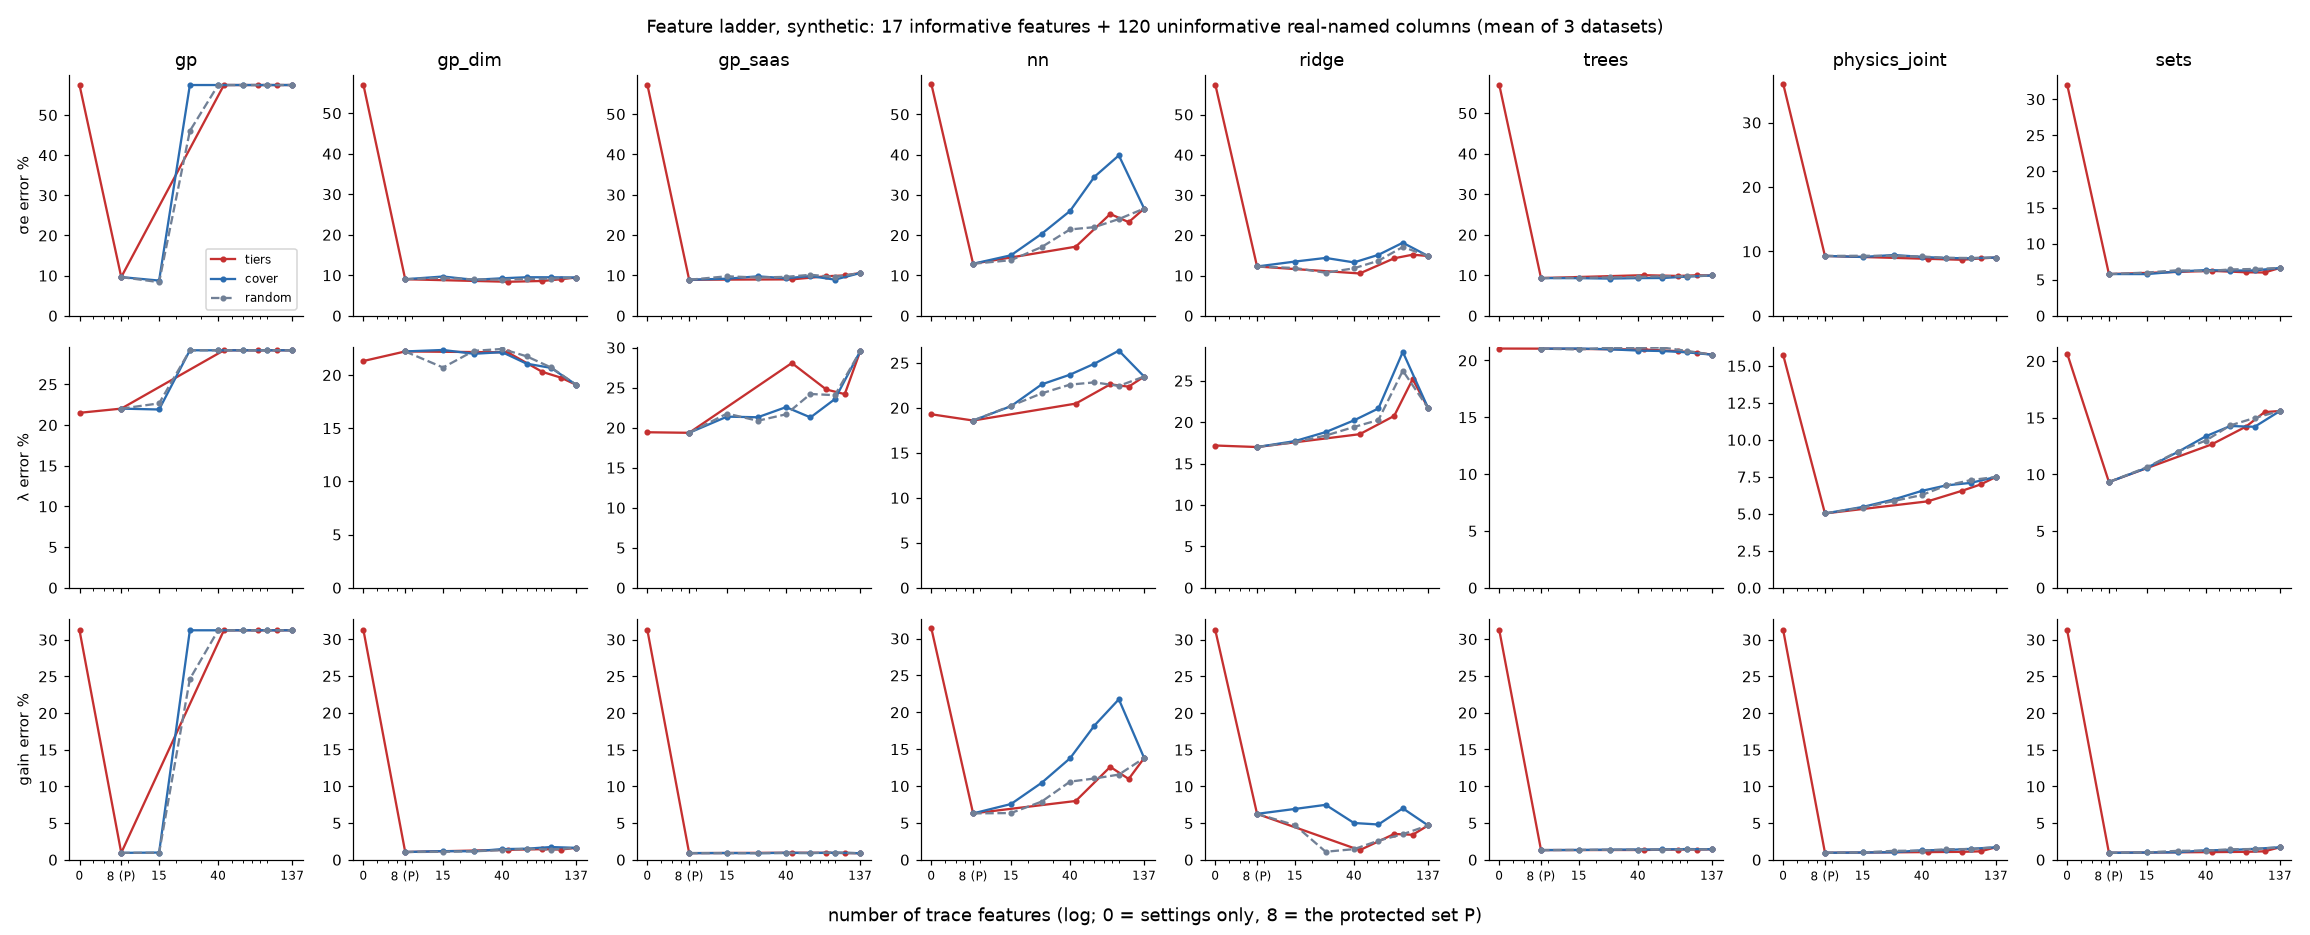
\includegraphics[width=\textwidth]{fig_feature_ladder.png}
\caption{The feature ladder on synthetic data: td41\_s0/1/2 with the 120 other real features added as uninformative
real-named columns; short training (\code{--quick}); mean of 3 datasets (\code{lvl1/feature\_study/ladder\_synthetic/}).}
\end{figure}

%======================================================================
\section{Commands}
\label{sec:cli}

\begin{verbatim}
# processing: one packet, or every packet with status ok
#   -> <out>/dataset.csv and <out>/model_inputs/
.venv/bin/python src/process_packet.py <manifest.json> \
    [--config configs/processing.toml]
.venv/bin/python src/process_packet.py --packets-dir <work_dir>/packets
cd src && ../.venv/bin/python -m ml.real_inputs <processed dir>   # inputs only

# synthetic test data in the same format
.venv/bin/python lvl1/make_test_data.py --out lvl1/test_data \
    --packets 100 --unlabeled 300

# train and score (default: ALL_MODELS, all features, 5 setting-grouped folds)
.venv/bin/python lvl1/train_lvl1.py --inputs <model_inputs> \
    [--models physics gp ...] [--quick] [--board 101] [--folds 5] \
    [--group-by setting|packet] [--setting-tol 0.01] [--n-boot 1000] \
    [--paired-ref physics] [--holdout-session C | --holdout-packets ID ...] \
    [--loao] [--feature-tiers all|none|auto|P+A...] \
    [--tier-ablation [SET ...]] [--ablation-ref SET] \
    [--feature-ladder [tiers cover random groups]] \
    [--ladder-steps 15 25 40 60 90] [--ladder-random 3] \
    [--tier-file lvl1/feature_study/evidence_tiers.json] \
    [--include-flagged] [--allow-fake] [--out DIR]

# evidence tiers (label-free) and learned importance (diagnostic)
.venv/bin/python lvl1/feature_study.py \
    [--data docs/slides/data/oct12_trace_features.csv]
.venv/bin/python lvl1/feature_importance.py --inputs <model_inputs> \
    [--add-noise 20] [--rounds 5] [--boot 30] [--repeats 5] [--saas]

# tests
.venv/bin/python -m unittest tests.test_lvl1_validation \
    tests.test_trace_features_new
\end{verbatim}

Outputs of \code{train\_lvl1.py}: \code{report.md} (tables per target, paired comparisons, ablation or ladder),
\code{report.json} (every score, interval and paired difference), \code{predictions.csv} (out-of-fold mean and sd per
model and target; held-out rows from the single fit), and \code{feature\_ladder.png} with the ladder.

%======================================================================
\section{Known limitations and open points in the code}
\label{sec:limits}

\paragraph{Limitations of the method.}
\begin{itemize}
  \item \textbf{Every result is synthetic.} The toy world's functional forms are invented; real packets (session A of the
        43-packet plan) are the first real test. Real data will also have 141 features instead of 17, so the
        feature-set defaults matter far more there.
  \item \textbf{$\lambda$ is the hardest label.} A trace holds almost no dark charge (10 pixels, $\sim$0.2\,s); in the
        toy world the dark current also follows a hidden state ($e^{0.35u}$) that the settings do not contain. Models that
        predict each amplifier from its own trace stay near the settings-only error for $\lambda$; the structured joint
        model does best. No protected (P) feature estimates $\lambda$.
  \item \textbf{The gain of a never-seen amplifier} cannot come from its trace (the trace measures $\sigma_1 g$); its
        absolute $\se$ in electrons needs one imaged packet.
  \item \textbf{Error bars:} the trees' quantile std under-covers (calibrated coverage is reported for every model); the
        conformal factor in the bootstrap is not re-estimated per resample.
  \item \textbf{Label-free tiers} reward separation, not prediction (hence the protected tier P); the learned tiers are
        diagnostics. Choosing among many feature sets on $\sim$30 packets is optimistic: choose on sessions A + B,
        confirm once on C.
\end{itemize}

\paragraph{Inconsistencies and possible bugs noticed while writing this reference.} Fixed on 2026-10-22: the packet state is
now amplifier-centred; the \code{ElasticNetCV} of \code{feature\_importance.py} uses packet-grouped folds; the Hadamard
deviation and the structure function are taken in log; the \code{process\_trace} docstring and the results table of
\code{lvl1/README.md} are updated; on 2026-10-23 \code{sets} got the SAAS GP for $\lambda$ ($\lambda$ 15.5 $\to$ 10.9,
10.9 $\to$ 7.4, 4.9 $\to$ 3.9\,\% at 13 / 41 / 100 packets, now equal to \code{physics}). Still open (behaviour changes, to decide):
\begin{enumerate}
  \item \textbf{\code{--quick} does not shorten \code{sets}} (\code{SetPooling}: 5 networks, 400 epochs) nor the SAAS chains
        of \code{physics} (fixed 96/48/8, by design).
  \item \textbf{Missing Allan curves:} \code{\_physics\_X} replaces NaN in the Allan array by the median of the
        \emph{whole} array (all rows, all $n$); a row with no curve then gets a flat curve and meaningless $(a, b)$
        instead of being flagged.
  \item \textbf{Early stopping of the networks} (\code{\_MeanVarHead}) uses a random 15\,\% of the training \emph{rows},
        not packets, as its validation split.
\end{enumerate}

\end{document}
